\documentclass[a4paper, 11pt]{article}

%%% SST LAB PROTOCOLL PREAMBLE
%%% 2019
%%%%%%%%%%%%%%%%%%%%%%%%%%%%%%%


%%% PACKAGES
%%%%%%%%%%%%%%%%%%%%%%%%%%%

\usepackage[ngerman]{babel}

\usepackage[utf8]{inputenc}
\usepackage{amsmath}
\usepackage{pgfplots}
\usepackage{tikz}
\usepackage[many]{tcolorbox}
\usepackage{graphicx}
\graphicspath{ {./graphics/} }
\usepackage{pdfpages}
\usepackage{dashrule}
\usepackage{float}
\usepackage{siunitx}
\usepackage{trfsigns}
\usepackage{booktabs}
\usepackage[european]{circuitikz}
\usepackage{tcolorbox}

%%% DOCUMENT GEOMETRY
%%%%%%%%%%%%%%%%%%%%%%%%%%%

\usepackage{geometry}
\geometry{
 a4paper,
 total={0.6180339887498948\paperwidth,0.6180339887498948\paperheight},
 top = 0.1458980337503154\paperheight,
 bottom = 0.1458980337503154\paperheight
 }
\setlength{\jot}{0.013155617496424828\paperheight}
\linespread{1.1458980337503154}

\setlength{\parskip}{0.013155617496424828\paperheight} % paragraph spacing


%%% COLORS
%%%%%%%%%%%%%%%%%%%%%%%%%%%

\definecolor{red1}{HTML}{f38181}
\definecolor{yellow1}{HTML}{fce38a}
\definecolor{green1}{HTML}{95e1d3}
\definecolor{blue1}{HTML}{66bfbf}
\definecolor{hsblue}{HTML}{00b1db}
\definecolor{hsgrey}{HTML}{afafaf}

%%% CONSTANTS
%%%%%%%%%%%%%%%%%%%%%%%%%%%
\newlength{\smallvert}
\setlength{\smallvert}{0.0131556\paperheight}


%%% COMMANDS
%%%%%%%%%%%%%%%%%%%%%%%%%%%

% differential d
\newcommand*\dif{\mathop{}\!\mathrm{d}}

% horizontal line
\newcommand{\holine}[1]{
  	\begin{center}
	  	\noindent{\color{hsgrey}\hdashrule[0ex]{#1}{1pt}{3mm}}\\%[0.0131556\paperheight]
  	\end{center}
}

% mini section
\newcommand{\minisec}[1]{ \noindent\underline{\textit {#1} } \\}

% quick function plot
\newcommand{\plotfun}[3]{
  \vspace{0.021286\paperheight}
  \begin{center}
    \begin{tikzpicture}
      \begin{axis}[
        axis x line=center,
        axis y line=center,
        ]
        \addplot[draw=red1][domain=#2:#3]{#1};
      \end{axis}
    \end{tikzpicture}
  \end{center}
}

% box for notes
\newcommand{\notebox}[1]{

\tcbset{colback=white,colframe=green1!100!black,title=Note!,width=0.618\paperwidth,arc=0pt}

 \begin{center}
  \begin{tcolorbox}[]
   #1 
  \end{tcolorbox}
 
 \end{center} 
 
}

% box for equation
\newcommand{\eqbox}[2]{
	
	\tcbset{colback=white,colframe=green1!100!black,title=,width=#2,arc=0pt}
	
	\begin{center}
		\begin{tcolorbox}[ams align*]
				#1
		\end{tcolorbox}
		
	\end{center} 
	
}
% END OF PREAMBLE

%%%%%%%%%%%%%%%%%%%%%%%%%%%%%%%%%%%%%

\begin{document}

%%%%%%%%%%%%%%%%%%%%%%%%%%%%%%%%%%%%%
  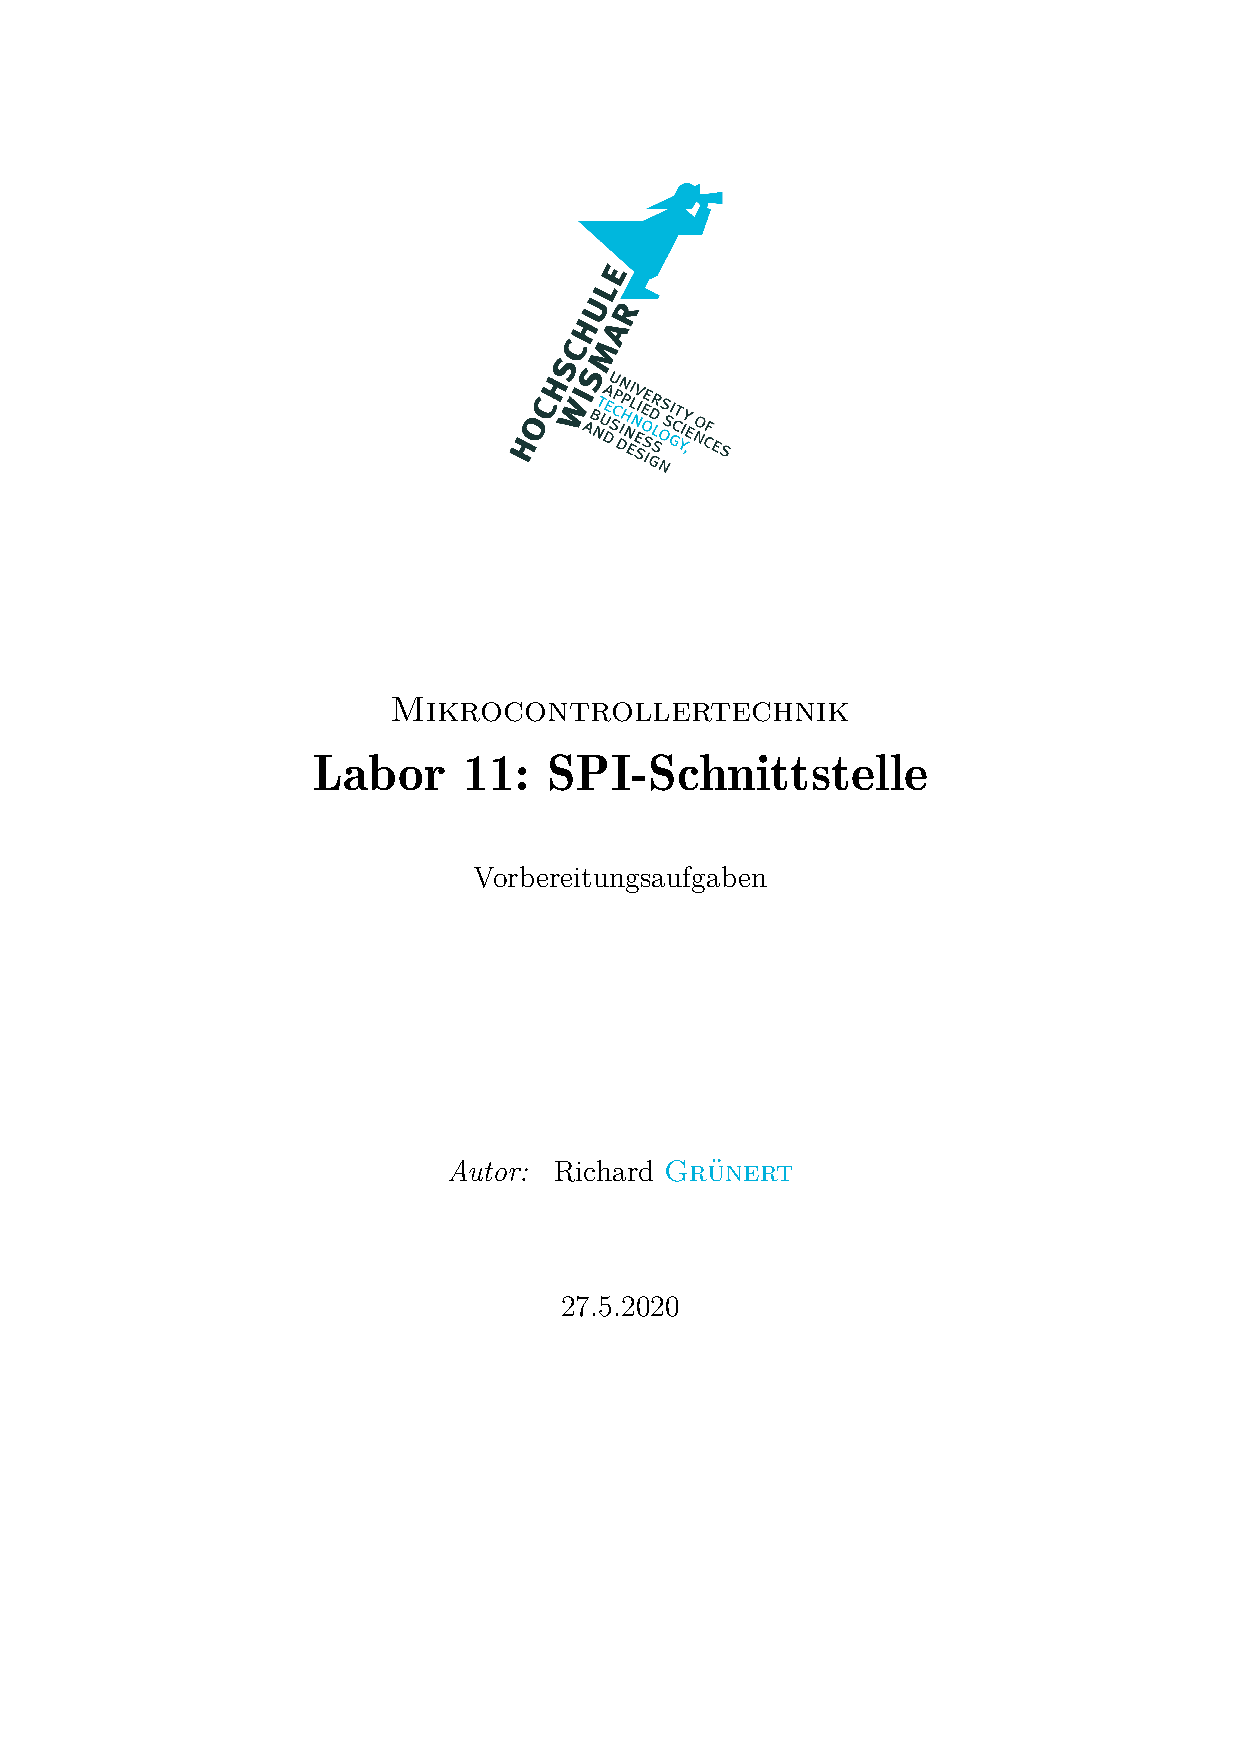
\includepdf{./titlepage/titlepage.pdf}
  \clearpage
  \setcounter{page}{1}
%%%%%%%%%%%%%%%%%%%%%%%%%%%%%%%%%%%%%

  \section{SPI-Datenübertragung}
  Die Datenübetragung mittels SPI erfolgt synchron mithilfe eines vom Master
  gesteuerten Taktes (SCLK) über die Datenleitungen MOSI (Master Out | Slave In)
  und MISO (Master In | Slave Out).

  \begin{figure}[H]
    \begin{center}
      \includegraphics[width=0.85410196625\textwidth]{SPI_basic}
  \end{center}
  \end{figure}
  \section{Signalfunktionen}
  \subsection{SCLK}
  Das $SCLK$ Signal dient der Taktung/Synchronisierung der Übertragung. Bei
  jeder fallenden Flanke geschieht eine Aktion, d.h. Senden/Empfangen am Master
  bzw. Empfangen/Senden am Slave.
  
  \subsection{MOSI}
  Master Out Slave In ($MOSI$, auch $SIMO$) ist die Sendedatenleitung des
  Masters. Intern wird ein Schieberegister parallel gefüllt, um seinen Inhalt
  dann seriell zu übertragen. Bei einer steigenden SCLK-Flanke wird das Datenbit angelegt und dann bei der
  fallenden gesendet.
  
  \subsection{MISO}
  Master In Slave Out ($MISO$, auch $SOMI$) ist die Empfangsdatenleitung des
  Masters. Intern wird ein Schieberegister seriell mit Empfangsdaten gefüllt, um
  dessen Inhalt dann parallel auszulesen.

  \subsection{SS / CS}
  Das Slave-Select-Signal ($\overline{SS}$) dient bei Kommunikation mit mehreren Slaves der
  Auswahl dieser durch den Master. Bei BUS-Verbindung der Slaves benötigt jeder
  Slave ein eigenes $\overline{SS}$ Signal, mit welchem er adressiert werden
  kann. Zieht der Master das jeweilige $\overline{SS}$ auf LOW wird die
  Empfangs- bzw. Sendefunktion des zugehörigen Slaves aktiviert.
  
  \section{Einstellung der Übertragungsgeschwindigkeit}
  Die Übertragungsgeschwindigkeit hängt von der SCLK-Rate ab. Die ausgewählte
  Taktquelle für SCLK kann über einen Prescaler geteilt werden.
  \[f_{\mathrm{BitClock}} = \frac{f_{\mathrm{BRCLK}}}{\mathrm{UCBRx}}\]

  \section{Vollduplexbetrieb}
  Im Vollduplexbetrieb können sowohl Daten vom Master gesendet (MOSI) als auch
  empfangen (MISO) werden. Die Daten werden jeweils in ein Schieberegister
  geschrieben, wodurch sie seriell bei jeder fallenden SCLK-Flanke gesendet/empfangen werden können.

\end{document}
% Local Variables:
% TeX-engine: luatex
% End:
